\chapter{Experiments}

In this chapter, we explain the setup of our experiments, describe how we measure the performance of different methods, and present the results.
All experiments were performed on a laptop with a 10-core, 16-thread Intel Core i7-12650H CPU and 32 GB of RAM. As for the software, Windows 11 24H2 was the operating system, MSVC 19.43 was the C++ compiler, and Python 3.12 was used.

\section{Datasets}

Here we briefly describe all datasets provided with the Google Hash Code Traffic signalling problem. This is important because the datasets have different sizes and structures.

\paragraph{A - An example: 4 parameters} Simple toy problem dataset used for debugging (See Figure~\ref{fig:hashcode_dataset_a}).

\paragraph{B - By the ocean: 5,974 parameters} Dataset based on a real city plan of Lisbon, Portugal (See Figure~\ref{fig:hashcode_dataset_b}).

\paragraph{C - Checkmate: 14,008 parameters} Dataset with a chessboard-like pattern and regular structure of intersections and streets (See Figure~\ref{fig:hashcode_dataset_c_e}).

% https://codeforces.com/blog/entry/88188#comment-765574
\paragraph{D - Daily commute: 167,748 parameters} By far the largest dataset with a challenging-to-navigate network from the \textit{Barabási-Albert} distribution.

\paragraph{E - Etoile: 1,386 parameters} Nicknamed \textit{Etoile}\footnote{\textit{Étoile} means star in French.}, this dataset is a one big star, meaning there is one very important intersection in the middle with hundrets of incoming streets (See Figure~\ref{fig:hashcode_dataset_c_e}).

\paragraph{F - Forever jammed: 10,002 parameters} Medium sized dataset but again with a complex network difficult to optimize.

\begin{figure}
    \centering
    % 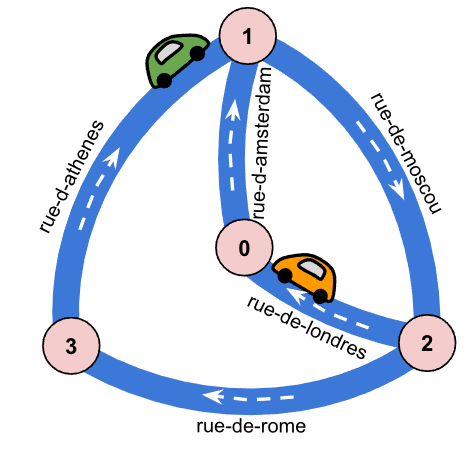
\includegraphics[width=\linewidth]{img/hashcode/figure5.png}
    % 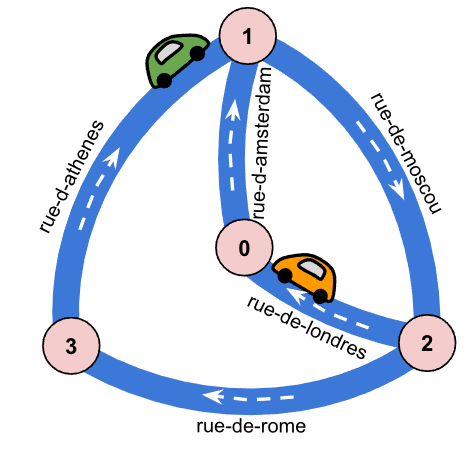
\includegraphics[width=.6\linewidth]{img/hashcode/figure5.png}
    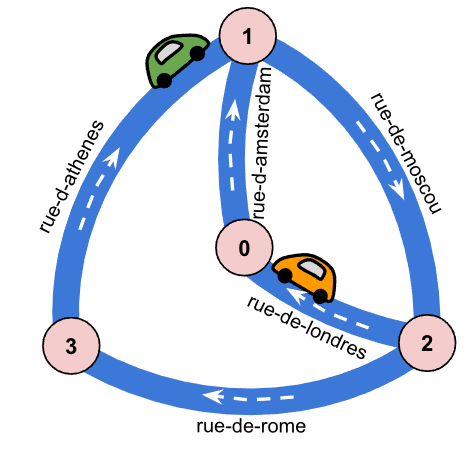
\includegraphics[width=.5\linewidth]{img/hashcode/figure5.png}
    \caption[Dataset A]{
        Dataset A \cite{google2023google}.
    }
    \label{fig:hashcode_dataset_a}
\end{figure}

\begin{figure}
    \centering
    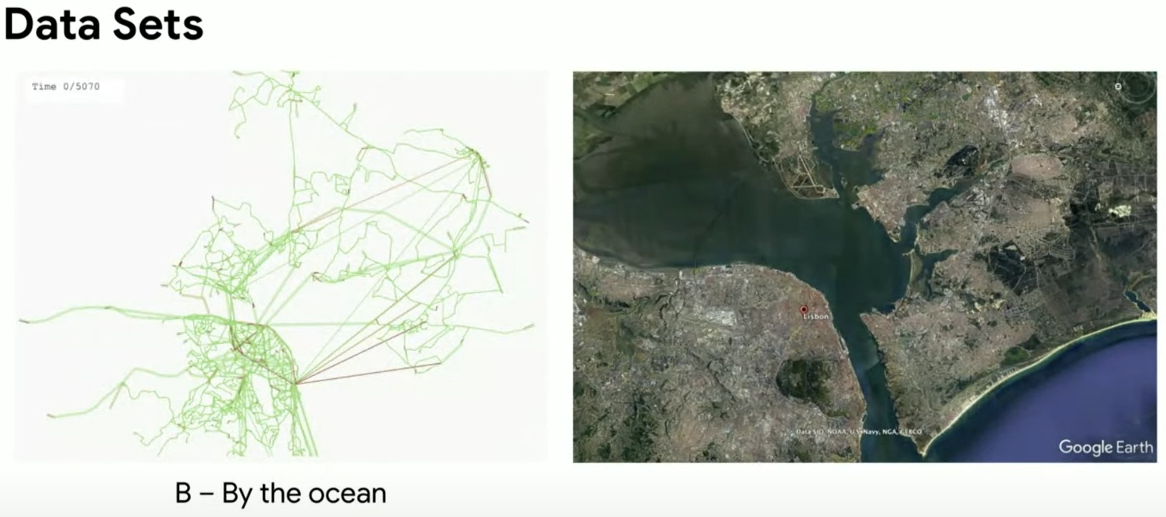
\includegraphics[width=\linewidth]{img/screenshots/hashcode_datasets_b.png}
    % 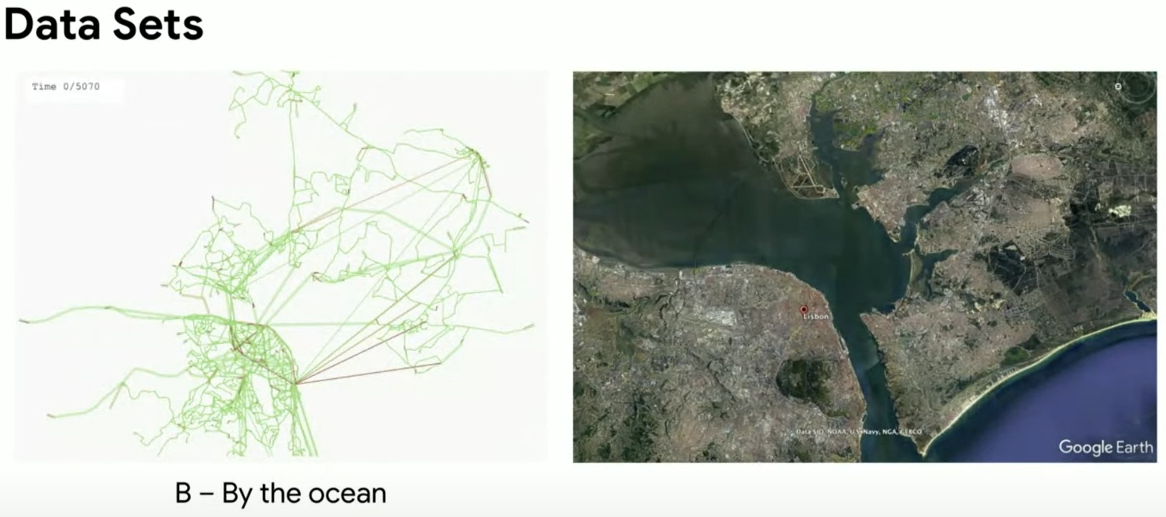
\includegraphics[width=.8\linewidth]{img/screenshots/hashcode_datasets_b.png}
    \caption[Dataset B]{
        Dataset B based on the real data of Lisbon on the right\footnotemark.
    }
    \label{fig:hashcode_dataset_b}
\end{figure}

\footnotetext{Screenshot from \href{https://www.youtube.com/watch?v=YPOVd-hQUjA}{Hash Code 2021: Online Qualification Round Livestream}.}

\begin{figure}
    \centering
    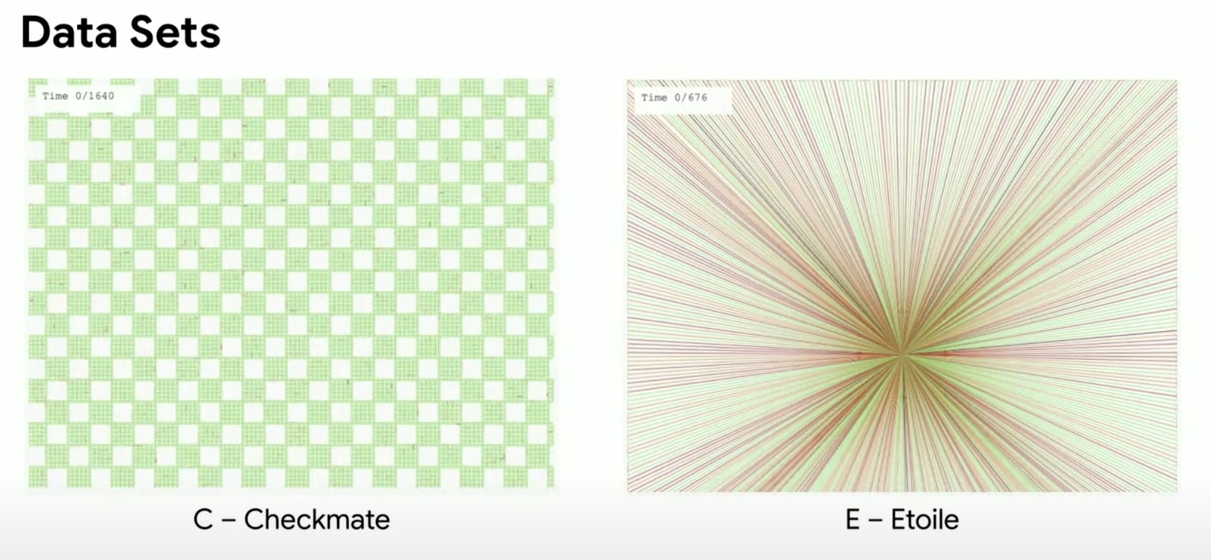
\includegraphics[width=\linewidth]{img/screenshots/hashcode_datasets_c_e.png}
    % 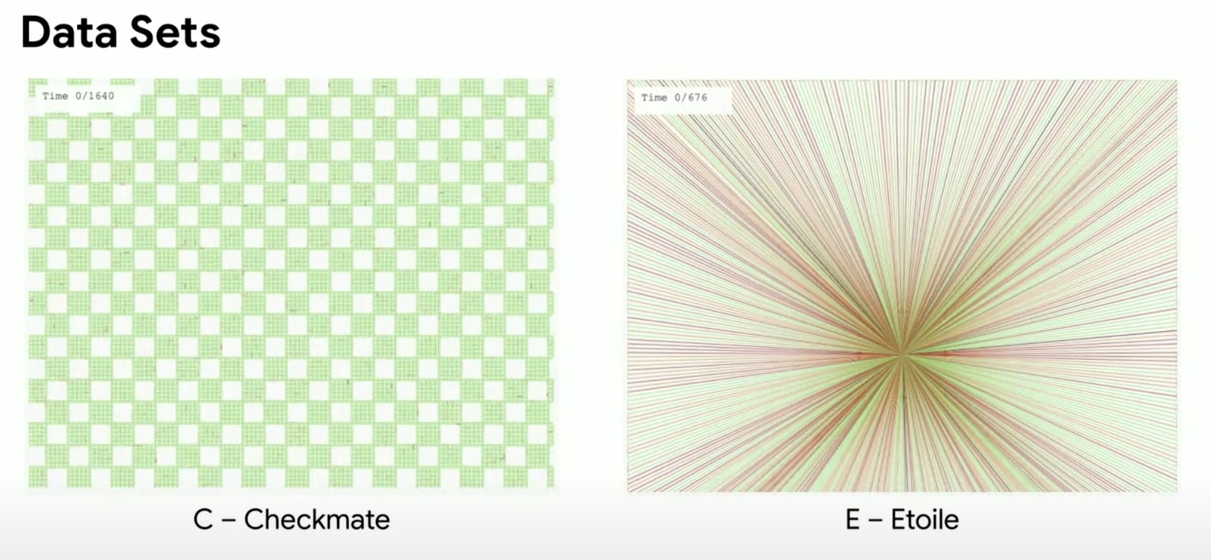
\includegraphics[width=.8\linewidth]{img/screenshots/hashcode_datasets_c_e.png}
    \caption[Datasets C and E]{
        Datasets C and E\footnotemark.
        }
        \label{fig:hashcode_dataset_c_e}
    \end{figure}
    
\footnotetext{See previous footnote.}

\bigskip

As previously stated, each dataset yields an absolute score in different range. To compare the performance across all datasets, we normalize the scores to a 0--1 range. 0 is a baseline solution with default order and default times and 1 is the maximum known score for the dataset. Note that the baseline is already a good solution and there may not be much room to improve further e.g., in dataset B.

\section{Experiment 1: Initialization}

\begin{figure}
    \centering
    % 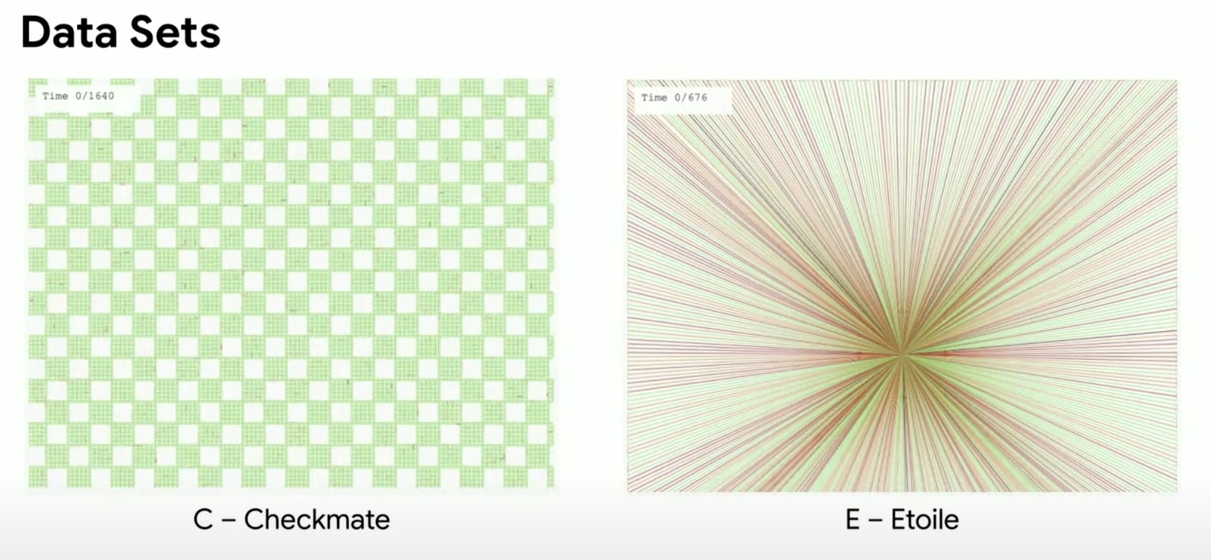
\includegraphics[width=\linewidth]{img/screenshots/hashcode_datasets_c_e.png}
    % 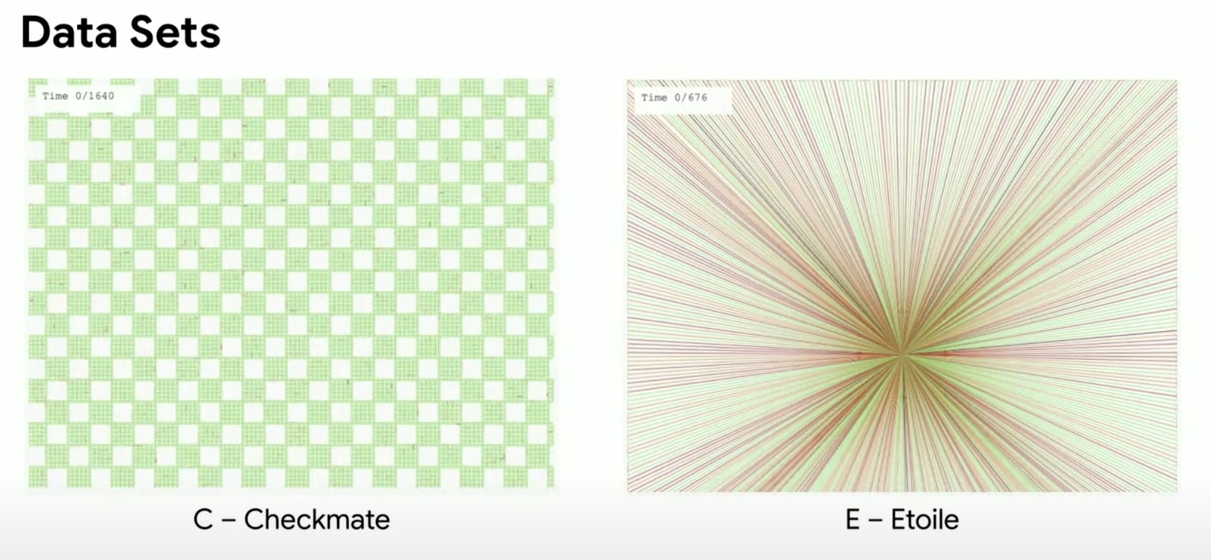
\includegraphics[width=.8\linewidth]{img/screenshots/hashcode_datasets_c_e.png}
    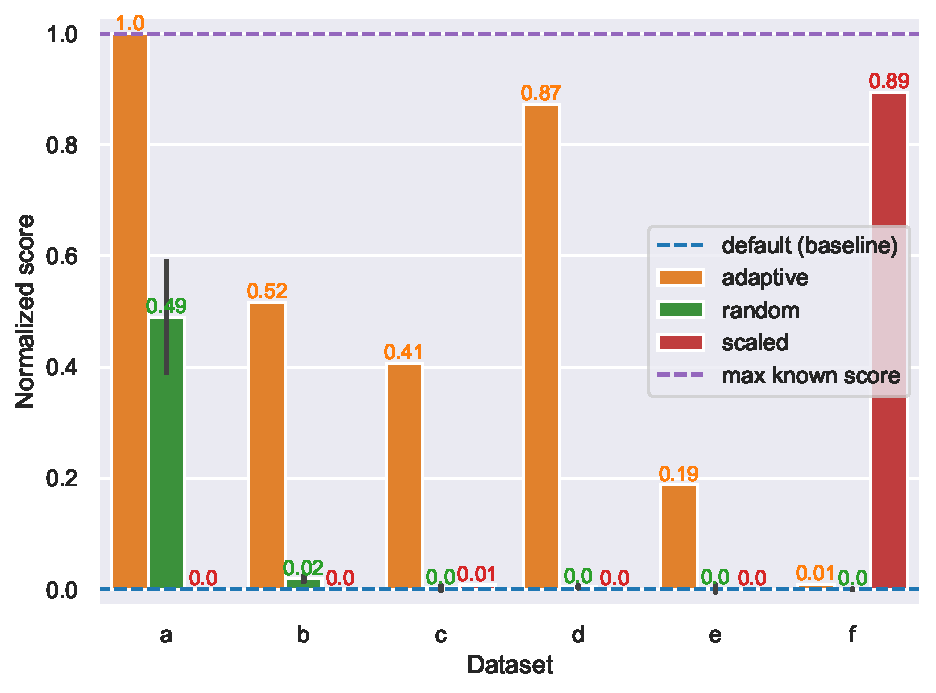
\includegraphics[width=\linewidth]{img/experiments/init_experiment.pdf}
    \caption[Initialization Experiment]{
        Initialization Experiment.
    }
    \label{fig:init_experiment}
\end{figure}

\section{Experiment 2: Optimization}
